\documentclass[12pt]{article}
\usepackage[utf8]{inputenc}
\usepackage[french]{babel}
\usepackage{graphicx}
\usepackage{listings}
\usepackage{float}
\usepackage{setspace}
\usepackage[colorinlistoftodos]{todonotes}

%Police
%\usepackage{helvet}
%\renewcommand{\familydefault}{\sfdefault}
%\usepackage[scaled]{arial}
%\renewcommand*\familydefault{\sfdefault} %% Only if the base font of the document is to be sans serif
\usepackage[T1]{fontenc}
\usepackage{amssymb}
\usepackage{verbatim}
\usepackage{amsmath}
\usepackage{multicol}

% ----------------------------------
\usepackage{algorithm}
\usepackage{algorithmic}
% ----------------------------------
\renewcommand{\algorithmicensure}{\textbf{Post-conditions :}}
\renewcommand{\algorithmicend}{\textbf{fin}}
\renewcommand{\algorithmicrequire}{\textbf{Pré-conditions :}}
\renewcommand{\algorithmicif}{\textbf{si}}
\renewcommand{\algorithmicthen}{\textbf{alors}}
\renewcommand{\algorithmicelse}{\textbf{sinon}}
\renewcommand{\algorithmicelsif}{\algorithmicelse\ \algorithmicif}
\renewcommand{\algorithmicendif}{\algorithmicend\ \algorithmicif}
\renewcommand{\algorithmicfor}{\textbf{pour}}
\renewcommand{\algorithmicforall}{\textbf{pour tout}}
\renewcommand{\algorithmicdo}{\textbf{faire}}
\renewcommand{\algorithmicto}{\textbf{jusqu'à}}
\renewcommand{\algorithmicendfor}{\algorithmicend\ \algorithmicfor}
\renewcommand{\algorithmicwhile}{\textbf{tant que}}
\renewcommand{\algorithmicendwhile}{\algorithmicend\
\algorithmicwhile}
\renewcommand{\algorithmicloop}{\textbf{boucler}}
\renewcommand{\algorithmicendloop}{\algorithmicend\
\algorithmicloop}
\renewcommand{\algorithmicrepeat}{\textbf{répéter}}
\renewcommand{\algorithmicuntil}{\textbf{jusqu'à}} 


% ----------------------------------
%\everymath{\displaystyle}

\title{Cahier des charges GSI}
\begin{document}



\begin{titlepage}

\newcommand{\HRule}{\rule{\linewidth}{0.5mm}} % Defines a new command for the horizontal lines, change thickness here

\center % Center everything on the page
 
%----------------------------------------------------------------------------------------
%	HEADING SECTIONS
%----------------------------------------------------------------------------------------

\textsc{\LARGE EISTI}\\[1.2cm] % Name of your university/college
\textsc{\Large Rapport Projet}\\[0.5cm] % Major heading such as course name
%\textsc{\large Les conférences}\\[0.5cm] % Minor heading such as course title

%----------------------------------------------------------------------------------------
%	TITLE SECTION
%----------------------------------------------------------------------------------------

\HRule \\[0.4cm]
{ \huge \bfseries Optimisation difficile pour des problème à variable continue}\\[0.4cm] % Title of your document
\HRule \\[1.5cm]
 
%----------------------------------------------------------------------------------------
%	AUTHOR SECTION
%----------------------------------------------------------------------------------------

\begin{minipage}{0.4\textwidth}
\begin{flushleft} \large
\emph{Auteurs:}\\
Elie \textsc{Poussou} \\
Ludovic \textsc{Lamarche} \\
Nicolas \textsc{Behra} \\
\end{flushleft}
\end{minipage}
~
\begin{minipage}{0.4\textwidth}
\begin{flushright} \large
\emph{Professeur:} \\
Rémi \textsc{Vernay} % Supervisor's Name
\end{flushright}
\end{minipage}\\[2cm]

% If you don't want a supervisor, uncomment the two lines below and remove the section above
%\Large \emph{Author:}\\
%John \textsc{Smith}\\[3cm] % Your name

%----------------------------------------------------------------------------------------
%	DATE SECTION
%----------------------------------------------------------------------------------------

{\large \today}\\[3cm] % Date, change the \today to a set date if you want to be precise

%----------------------------------------------------------------------------------------
%	LOGO SECTION
%----------------------------------------------------------------------------------------


\includegraphics[scale=.25]{EISTI.jpg}\\[1cm] % Include a department/university logo - this will require the graphicx package
 
%----------------------------------------------------------------------------------------

\vfill % Fill the rest of the page with whitespace

\end{titlepage}
\renewcommand{\contentsname}{Sommaire}
\doublespacing
\tableofcontents
\singlespacing

\newpage

%Essaim.h Nicolas
%Abeille.h Ludo
%Test.cpp Elie

%TODO
%Commentaire
%Enlever parametre inutile dans essaim Nico
%Supprimer code inutile ---
%Ré-organiser les test ----- Elie
%OpenMP abeille ----- Ludo
%Un readme ------
%Mettre le nombre d'itérations dans les abeilles en paramètre ---- Ludo

\section*{Introduction} %Elie

Dans le cadre de notre 3ème semestre de cycle ingénieur, il a été proposé aux élèves du parcours GSI un projet dont le but est de créer une librairie permettant d'effectuer une optimisation difficile pour des problèmes à variable continue.

Le but de cette librairie est de trouver la solution à des fonctions difficiles en un temps réduit.

Pour mener à bien ce projet et résoudre ces problèmes, il nous a été proposé des heuristiques qui sont des méthodes pour trouver des solutions à des problèmes difficiles. 

Dans un premier temps, nous avons travaillé sur le fonctionnement de ces différentes heuristiques dans le cahier des charges.

Dans ce rendu final, nous allons tout d'abord expliquer comment nous avons adapté les deux heuristiques choisies pour les faire fonctionner dans notre cas.
En effet, notre librairie peut fonctionner avec l'heuristique des essaims particulaires ou avec celle des colonies d'abeilles artificielles. 

Ensuite, nous allons expliquer comment un développeur souhaitant utiliser notre librairie peut le faire en fonction de l'heuristique choisie.

Enfin, une comparaison des performances en fonction de l'heuristique choisie sera présentée.

Cette librairie pourra fonctionner sur un seul ordinateur en mode séquentiel ou sur plusieurs ordinateurs en mode parallèle. 

\newpage
\section{Modifications d'algorithme}

\subsection{Heuristique des abeilles}
Concernant l'heuristique des abeilles, nous avions présenté le déroulement de cette méthode mais nous n'avions pas précisément d'algorithme. \\
Voici ci dessous l'algorithme final utilisé pour implémenter cette heuristique.
\begin{algorithm}
 \caption{Algorithme des colonies d'abeilles artificielles}
 
 \begin{algorithmic}
 \STATE{\textbf{res}=une fleur très mauvaise}
 	\FOR{$i = 1 $ \TO $max_iterations$}
     \STATE{mise a jour des fitness}
      \FOR{chaque observatrice}
      	\STATE{\textbf{fleur} = choisir une fleur aléatoirement}
        \STATE{fleur->nbIterations=fleur->nbIterations+1}
        \STATE{\textbf{voisin}=générer une fleur voisine à \textbf{fleur}}
        
       	 \indent \textbf{si} fitness(\textbf{voisin})>fitness(\textbf{fleur})\textbf{faire}\\
         	\indent \indent \textbf{fleur}<-\textbf{voisin}\\
            \STATE{\textbf{fleur}->nbIterations=0}
         \textbf{finsi}
         	\STATE{\textbf{si} fitness(\textbf{fleur})>fitness(\textbf{res})}
            	\indent \STATE{res=\textbf{fleur}}
               \STATE{\textbf{fin si}}
         	
      \ENDFOR
    \ENDFOR
    \STATE{retourner \textbf{res}}
 	
 \end{algorithmic}
\end{algorithm}
\subsection{Heuristique des essaims}
Après implémentation de l'algorithme des essaims particulaires avec voisinage, fourni dans le premier rapport, nous avons dû adapter de manière empirique cet algorithme pour un fonctionnement et une efficacité optimale.

     \newpage
    Après étude et application de cet algorithme sur des fonctions objectifs concrètes telles que la fonction carré ou encore la fonction de Bohachevsky \cite{fonctionsObjectifs}. Les principales modifications se sont faites au niveau du calcul de la nouvelle vitesse. 
   
    Précédemment on calculait la nouvelle vitesse ainsi:\\
    

    $ v_{i} \leftarrow \kappa (v_{i} + \rho_{1} (x_{p_{i}} - x_{i}) + \rho_{2} (x_{v_{i}} - x_{i}) $ \\
    avec: 
    \begin{itemize}
      \item \textit{ $x_{i}$ } : la position de cette particule dans l'espace;
      \item \textit{ $v_{i}$ } : sa vitesse;
      \item  \textit{ $x_{p_{i}}$ } : position par laquelle elle est déjà passée et dont la solution est la meilleure; 
      \item  \textit{ $x_{v_{i}}$ } : position du voisin pour laquelle la solution est la meilleure; 
      \item $ \kappa = 1 - \frac{1}{\rho} + \frac{\sqrt{ |\rho^2 - 4\rho|}}{2} $
      \item $\rho = \rho_{1} + \rho_{2} > 4$
      \item $\rho_{1} = r_{1}*c_{1}$
      \item $\rho_{2} = r_{2}*c_{2}$ 
	\end{itemize}
    
    
    
Où $c_{1}$, $c_{2}$  sont deux constantes positives déterminées de façon empirique et telles que $c_{1} + c_{2} \le 4 $ et $r_{1}, r_{2}$ suivent une loi uniforme sur [0..1]. \\
  Nous évoquions aussi le fait que la fonction de constriction devait être comprise entre $0.8$ et $1.2$ pour une convergence optimale d'où la nouvelle vitesse est calculée comme suit: \\
    
    $ v_{i} \leftarrow c1 * v_{i} + R * (x_{p_{i}} - x_{i}) + (1-R) * (x_{v_{i}} - x_{i}) $
    
    avec $c1$: variable aléatoire entre $0.8$ et $1.2$;\\
    $R$: variable aléatoire entre $0$ et $1$. \\
    
    Ici, on doit comprendre que la vitesse peut accélérer, décélérer ou bien même stagner c'est pourquoi on multiplie la vitesse précédente par c1. Puis on simule la tendance d'une particule à suivre son instinct ou à suivre ses voisins par la variable $R$. 
    

\section{API}

\subsection{Fonction Objectif}
Pour la création d'une nouvelle fonction Objectif, il faut créer une classe qui contient, les méthodes getMin(), getMax(),et la formule de la fonction Objectif.

  \begin{lstlisting}
    double f(const std::vector<double> params) const;
  \end{lstlisting}
    \begin{itemize}
      \item params les paramètres de la fonction
      \item  retourne l'image des paramètre par la fonction objectif
    \end{itemize}
  \begin{lstlisting}
  	std::vector<double> getMin()const;
  \end{lstlisting}
  \begin{lstlisting}
	std::vector<double> getMax()const;
  \end{lstlisting}
  Ces deux méthodes permettent respectivement de fournir les bornes min et les bornes max de la fonction objectif correspondante.
  
  Au vu de notre implémentation on peut créer des fonctions objectifs avec autant de dimensions que l'on souhaite.
  

\subsection{Constructeur Abeille}
\begin{lstlisting}
Abeille(F _obj, unsigned _nbFleurs, unsigned _iterationMaxParFleur,
	unsigned _maxIteration);
\end{lstlisting}
\begin{itemize}
	\item \_obj Objet contenant une fonction objectif f(vector<double> v), getMin() et getMax() pour donner les bornes de cette fonction
    \item  \_nbFleurs le nombre de fleur souhaité pour l'exécution de l'algorithme
    \item \_iterationMaxParFleur le nombre de fois qu'une abeille observatrice passe sur une fleur avant de la laisser tomber
    \item \_maxIteration le nombre d'itération total de l'algorithme
    \end{itemize}
    
\newpage
\subsection{Constructeur Essaim}
\begin{lstlisting}
   Essaim(F _obj, unsigned _nbParticules, unsigned _cArret);
  \end{lstlisting}
  \begin{itemize}
      \item \_obj Objet contenant une fonction objectif f(vector<double> v), getMin() et getMax() pour donner les bornes de cette fonction
      \item  \_nbParticules le nombre de particule souhaité pour l'exécution de l'algorithme
      \item \_cArret la condition d'arrêt, c'est à dire le nombre maximum d'itération.
  \end{itemize}

\subsection{Solve}
\begin{itemize}
\item solve : permet de lancer l'algorithme en parallélisant
\item solve(unsigned n) : permet de lancer l'algorithme en utilisant n threads.
\item solveMpi(const MpiBind \&mpi) : parallélise en utilisant MPI, le résultat sera mis à jour dans l'objet du thread 0
\end{itemize}

\begin{lstlisting}
Fschwefel<3> f;
Abeille<Fschwefel<3>> e(f, 100, 1000, 10000);
e.solveMpi(mpi); //Execution MPI
if (mpi.getRank() == 0) {
cout << "MPI :" << e << endl; //Resultat sur le thread 0
}
e.solve(3); //Execution parallele
e.solve(1); //Execution non parallele
\end{lstlisting}


\subsection{GetResultat}
Permet de récupérer la position minimum de la fonction après l'exécution de solve.
\begin{lstlisting}
std::vector<double> Abeille<F>::getResultat() const;
\end{lstlisting}

\newpage
\subsection{Flux de sortie <<}
Vous pouvez afficher le résultat sous la forme $F(x)=y$ en utilisant le flux de sortie sur l'objet après avoir appliqué solve.
\begin{lstlisting}
Fschwefel<3> f;
Abeille<Fschwefel<3>> e(f, 100, 1000, 10000);
e.solve();
cout << e << endl;
\end{lstlisting}


\subsection{Exemple}
\begin{lstlisting}
Fbohachevsky f { };
Abeille<Fbohachevsky> abeille(f,500,100,10000);
abeille.testGenererFleur();

Fbohachevsky f { };
Essaim<Fbohachevsky> e(f,100,10000);
e.testGenererFleur();
\end{lstlisting}

\subsection{Exécution des tests}
Pour exécuter les test en utilisant openmp, il y a deux options possible :
\begin{itemize}
\item -a : exécute les tests sur les abeilles
\item -e : exécute les tests sur les essaims
\end{itemize}
\begin{lstlisting}
$./Debug/projetgsi
    $./Debug/projetgsi -a
    $./Debug/projetgsi -e
\end{lstlisting}
Pour désactiver le multithreading, il faut mettre la variable d'environnement OMP\_GET\_NUM\_THREADS à 1.\\
Pour tester MPI :
\begin{lstlisting}
	$mpirun -np 4 ./Debug/projetgsi
\end{lstlisting}


\newpage
%Elie
\section{Tests expérimentaux}
Pour tester les différentes solutions de notre librairie, nous avons utilisé différentes fonctions en 1,2 et 3 dimensions. 

Les fonctions que nous avons testés ont beaucoup de variations et donc beaucoup de minimums locaux, par exemple les deux fonctions suivantes.
\begin{multicols}{2}
   \begin{figure}[H]
	\centering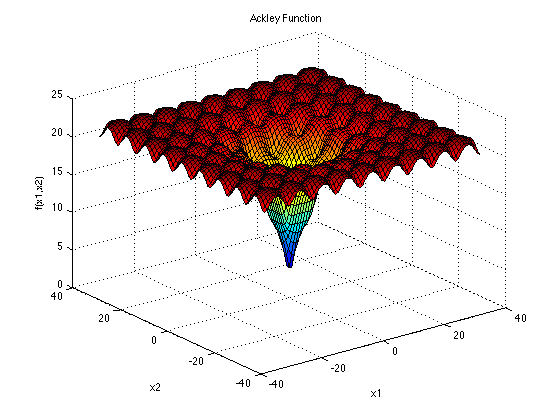
\includegraphics[scale=0.35]{ackley.png}
    \caption{Fonction de Ackley}
\end{figure}
   
   \begin{figure}[H]
	\centering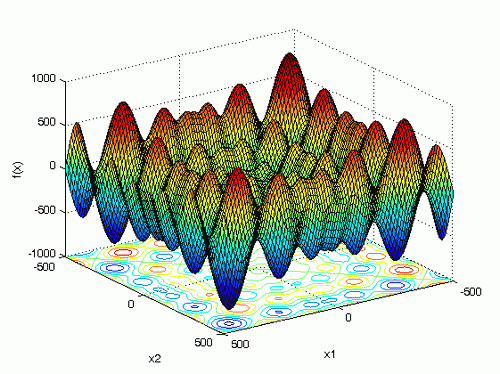
\includegraphics[scale=0.35]{schwefel.png}
    \caption{Fonction de Schwefel}
\end{figure}
\end{multicols}
\begin{figure}[H]
	\centering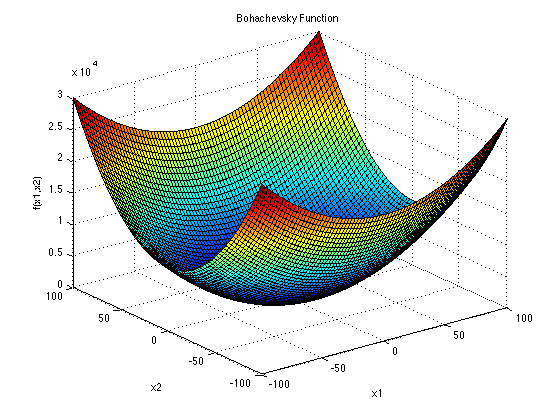
\includegraphics[scale=0.35]{boha.png}
    \caption{Fonction de Bohachevsky}
\end{figure}

\newpage
\vspace*{2cm}
Nous avons noté des différences entre les performances des 2 algorithmes, nous avons récapitulé ces différences dans le tableau suivant : 
\\

\begin{tiny}

\noindent\begin{tabular}{|*{4}{c|}}
    \hline
     & Essaim & Abeille & resultat attendu \tabularnewline
     \hline
   F carré& F(-4.4*$10^{-9}$) = 1.9*$10^{-17}$
& F(-5.4*$10^{-6}$) = 2.9*$10^{-11}$ & F(0)=0
\tabularnewline
    \hline
    Ackley & F(-5.9 *$10^{-4}$,3.4*$10^{-4}$) = 1.9*$10^{-3}$
    & F(-1.4*$10^{-2}$,5.7*$10^{-2}$) = 4.8*$10^{-2}$ & F(0,0)=0  \tabularnewline
    \hline
    Bohachevsky & F(-6.4*$10^{-4}$,$10^{-3}$) = 4.6*$10^{-5}$ &
    F(8.3*$10^{-2}$,-9.6*$10^{-2}$) = 0.3 resultat boha abeille & F(0,0)=0 
    \tabularnewline
    \hline
    Schwefel & F(420.969,420.969,420.969) = 3.8*$10^{-5}$ & 
    F(421.673,420.704,421.028,) = 7.2*$10^{-2}$& F(420.969,420.969,420.969)=0
    \tabularnewline
    \hline

    
 \end{tabular}
\end{tiny}
\newline

La différence de précision entre les deux algorithmes est flagrante, même pour une fonction assez simple comme la fonction carrée, on observe une différence de 3 chiffres après la virgule. 

Cette différence se maintient sur les 3 autres fonctions.

Néanmoins, même si il est difficile de comparer les temps d'exécution car il dépend des différents paramètres de l'algorithme comme le nombre d'itérations par exemple, on observe que l'algorithme des abeilles est à peu près 2 fois plus rapide.
\newline
\newline
Finalement, si l'on veut privilégier la vitesse d'exécution, on peut utiliser l'algorithme des abeilles qui donne quand même une bonne idée de la solution exacte.

Si l'on veut privilégier la précision, il faudra utiliser l'heuristique des essaims qui renverra des résultats plus proches de la solution exacte. 

\newpage
\section*{Conclusion}%Conclusion

L'étude des comportements animaliers nous permet d'en déduire des algorithmes pouvant être utilisés dans le cadre d'optimisation difficile de fonctions dites objectifs. Après implémentation avec parallélisation on peut en tirer plusieurs conclusions, l'algorithme des essaims particulaires est plus optimal en terme de précision que l'algorithme des Abeilles bien que ce dernier soit plus rapide. De la manière dont on a implémenté la parallélisation, côté mpi ce n'est pas plus rapide mais le résultat est un peu plus précis et côté openmp on observe une exécution plus rapide remarquable.



\nocite{*}
\bibliographystyle{unsrt}
\bibliography{biblio}

\end{document}